% Chattering Comparison: Classical SMC vs. STA
% TikZ diagram for Chapter 4

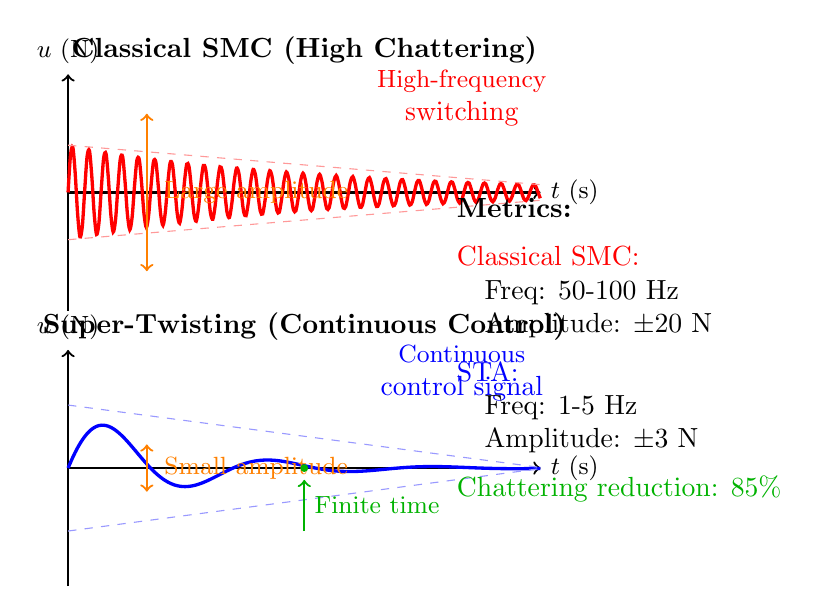
\begin{tikzpicture}[scale=1.0]

    % Classical SMC subplot (top)
    \begin{scope}[yshift=3.5cm]
        % Axes
        \draw[->, thick] (0, 0) -- (6, 0) node[right] {\small $t$ (s)};
        \draw[->, thick] (0, -1.5) -- (0, 1.5) node[above] {\small $u$ (N)};

        % Title
        \node[above] at (3, 1.5) {\textbf{Classical SMC (High Chattering)}};

        % High-frequency oscillations
        \draw[red, very thick, samples=200, smooth, domain=0:6]
            plot ({\x}, {0.6*exp(-0.3*\x)*sin(30*\x r)});

        % Envelope
        \draw[red!40, dashed] (0, 0.6) -- (6, {0.6*exp(-1.8)});
        \draw[red!40, dashed] (0, -0.6) -- (6, {-0.6*exp(-1.8)});

        % Annotation
        \node[red, align=center] at (5, 1.2) {\small High-frequency\\switching};
        \draw[<->, thick, orange] (1, -1) -- (1, 1);
        \node[orange, right] at (1.1, 0) {\small Large amplitude};
    \end{scope}

    % STA subplot (bottom)
    \begin{scope}
        % Axes
        \draw[->, thick] (0, 0) -- (6, 0) node[right] {\small $t$ (s)};
        \draw[->, thick] (0, -1.5) -- (0, 1.5) node[above] {\small $u$ (N)};

        % Title
        \node[above] at (3, 1.5) {\textbf{Super-Twisting (Continuous Control)}};

        % Smooth exponential convergence
        \draw[blue, very thick, samples=100, smooth, domain=0:6]
            plot ({\x}, {0.8*exp(-0.8*\x)*sin(3*\x r)});

        % Envelope
        \draw[blue!40, dashed] (0, 0.8) -- (6, {0.8*exp(-4.8)});
        \draw[blue!40, dashed] (0, -0.8) -- (6, {-0.8*exp(-4.8)});

        % Annotation
        \node[blue, align=center] at (5, 1.2) {\small Continuous\\control signal};
        \draw[<->, thick, orange] (1, -0.3) -- (1, 0.3);
        \node[orange, right] at (1.1, 0) {\small Small amplitude};

        % Convergence marker
        \fill[green!70!black] (3, 0) circle (0.05);
        \draw[->, thick, green!70!black] (3, -0.8) -- (3, -0.15)
            node[midway, right] {\small Finite time};
    \end{scope}

    % Comparison metrics
    \begin{scope}[xshift=7cm, yshift=1.5cm]
        \node[align=left] at (0, 0) {
            \textbf{Metrics:}\\[0.2cm]
            \textcolor{red}{Classical SMC:}\\
            \quad Freq: 50-100 Hz\\
            \quad Amplitude: $\pm20$ N\\[0.2cm]
            \textcolor{blue}{STA:}\\
            \quad Freq: 1-5 Hz\\
            \quad Amplitude: $\pm3$ N\\[0.2cm]
            \textcolor{green!70!black}{Chattering reduction: 85\%}
        };
    \end{scope}

\end{tikzpicture}
